\subsubsection{Regressione lineare}
\fancyhead{}    % reset header
\fancyhead[R]{Regressione lineare}
\label{paragrafo 4.2.1}
Una volta definito il processo di feature engineering e scelte le tecniche di valutazione, è
stato possibile definire un modello di regressione lineare tramite la libreria \textit{sklearn.linearmodel},
in particolare si è utilizzato il metodo \textit{fit} per addestrare il modello sull’insieme dei dati di
training e in seguito \textit{predict} sull’insieme dei dati di test per predirne il valore della variabile
dipendente basandoci sulle feature dell’insieme di dati di training.
Prima di procedere con la creazione del modello di regressione lineare multipla, abbiamo
verificato che i nostri dati rispettassero le condizioni di:
\par{
\begin{itemize}
    \item \textbf{Linearità dei dati}
    \begin{figure}[H]
        \centering
        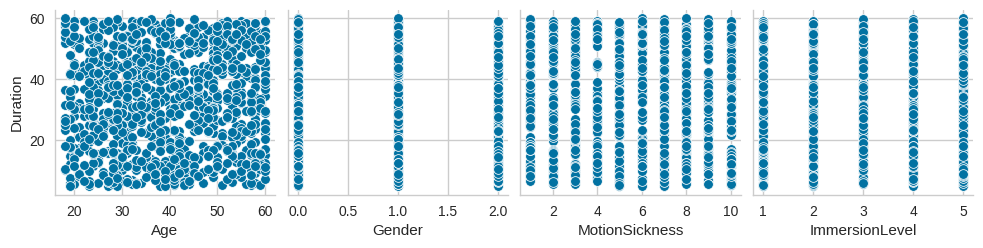
\includegraphics[width=1\linewidth]{image.png}
        \caption{Linearità dei dati}
        \label{fig:enter-label}
    \end{figure}
    da come si nota in figura, si hanno dei dati che hanno una distribuzione omogenea e lineare rispetto alla variabile dipendente \textit{Duration}.
    \item \textbf{Bassa multicollinearità}
    \begin{figure}[H]
        \centering
        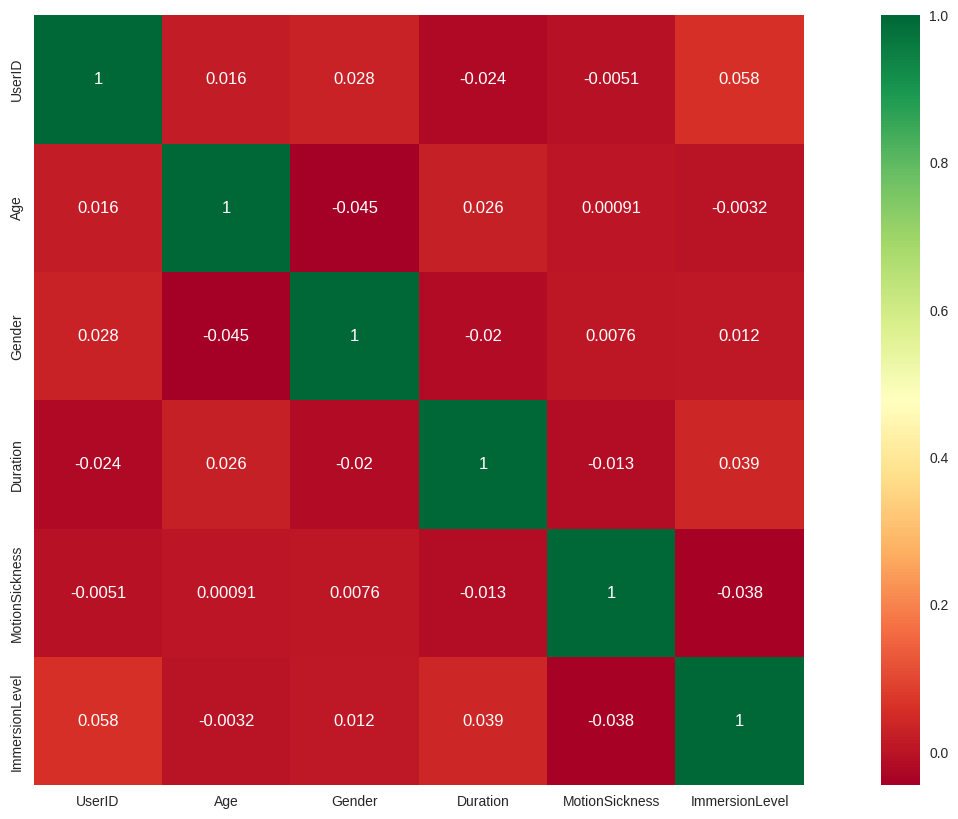
\includegraphics[width=1\linewidth]{multicoll.png}
        \caption{Multicollinearità}
        \label{fig:enter-label}
    \end{figure}
    in quest'altra figura invece si nota che le feature utilizzate nel dataset non sono fortemente correlate tra loro, quindi consente al modello di applicare una regressione lineare multipla senza preoccuparsi di avere variabili ridondanti durante l'addestramento.
\end{itemize}
}

Al fine di definire il modello che si adatti meglio i dati, è stato necessario applicare il \textbf{metodo empirico}, cioè l'utilizzo di vari algoritmi di regressione al fine di trovare quello più adatto al problema in esame.\\
Per ogni modello creato, sono stati applicate 3 diverse tipologie di normalizzazione del dataset per poter scegliere in modo più accurato il modello da utilizzare. Le 3 normalizzazioni sono:
\par{
\begin{itemize}
    \item \textbf{Z-Score normalization}\\
    \begin{equation}
        Z = \frac{x - \mu}{\sigma}
    \end{equation}
    \item \textbf{MinMax normalization}
    \begin{equation}
        X_{\text{norm}} = \frac{X - X_{\text{min}}}{X_{\text{max}} - X_{\text{min}}}
    \end{equation}
    \item \textbf{Robust scaling}
    \begin{equation}
        X_{\text{robust}} = \frac{X - \text{Mediana}}{\text{IQR}}
    \end{equation}
\end{itemize}
}\\

Infine, oltre alle 3 metriche descritte nel paragrafo \ref{paragrafo 4.1}, per poter valutare la validità delle stime è stato fatto un controllo e un plot dei \textbf{residui} ricavati durante l'esecuzione del modello sul \textit{test set}. \\
Più in dettaglio abbiamo verificato:
\par{
\begin{itemize}
    \item \textbf{normalità dei residui}: se i residui vengono \textbf{normalmente distribuiti} cioè se i residui seguono o meno una distribuzione approssimativamente normale. Si guarda se la forma della distribuzione è a campana simmetrica.
    \item \textbf{omoschedasticità}: se gli errori residui hanno una varianza \textbf{costante}, cioè commettono un tasso di errore costante.
    \begin{figure}[H]
        \centering
        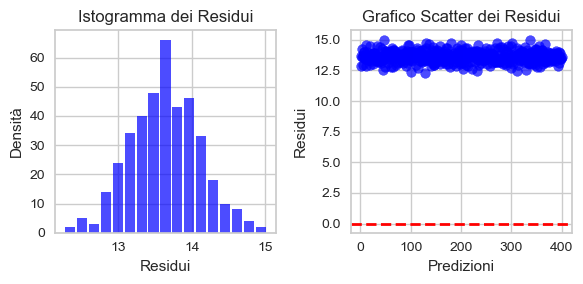
\includegraphics[width=1\linewidth]{plotresidui.png}
        \caption{Esempio di plot dei residui}
        \label{fig:enter-label}
    \end{figure}
\end{itemize}
}

Partendo dalle metriche è stata deinita una semplice classe che contesse 3 array di tutte le metriche ricavate durante la fase di validazione: \\
\begin{lstlisting}[caption=Classe Metrics1]
#oggetto che contiene le metriche
class Metrics1:
  #costruttore
  def __init__(self,mae,mse,rmse):
    self.mae=mae      #MAE
    self.mse=mse      #MSE
    self.rmse=rmse    #RMSE

  #ToString
  def __str__(self):
    return f'Metrics [mae= {self.mae} mse= {self.mse} rmse= {self.rmse} mean= {np.mean([self.mae,self.mse,self.rmse])}'
\end{lstlisting} 

Tale classe è servita definire MetricsResultContainer, un ulteriore classe che funge da "ambiente" per poter eseguire metodi specifici sul plot dei residui e sulla stampa delle metriche in base al modello e alla tipologia di normalizzazione utilizzata: \\
\begin{lstlisting}[caption=MetricsResultContainer]

class MetricsResultContainer:
    meanMAE = []
    meanMSE = []
    meanRMSE = []

    def __init__(self, model, alg, scaler, param, metricsMean):
        self.model = model
        self.alg = alg
        self.scaler = scaler
        self.param = param
        self.metricsMean = metricsMean
        self.meanMAE = []
        self.meanMSE = []
        self.meanRMSE = []
        

    def printMetrics(self):
        for m in self.metricsMean:
            self.meanMAE.append(m.mae)
            self.meanMSE.append(m.mse)
            self.meanRMSE.append(m.rmse)
        print("meanMAE=", np.mean(self.meanMAE))
        print("meanMSE=", np.mean(self.meanMSE))
        print("meanRMSE=", np.mean(self.meanRMSE))
        
        self.visualizza_grafici()
        self.test_Durbin_Watson()

    # funzione per mostrare la normalità dei residui e l'omoschedasticità
    def visualizza_grafici(self):
        fig, axs = plt.subplots(1, 2, figsize=(6, 3))  # Una riga, due colonne

        # Istogramma dei Residui
        axs[0].hist(self.meanMAE, bins='auto', color='blue', alpha=0.7, rwidth=0.85)
        axs[0].set_title('Istogramma dei Residui')
        axs[0].set_xlabel('Residui')
        axs[0].set_ylabel('Densità')

        # Grafico Scatter dei Residui
        lunghezza_dati = len(self.meanMAE)
        axs[1].scatter(np.arange(1, lunghezza_dati + 1), self.meanMAE, color='blue', alpha=0.7)
        axs[1].axhline(y=0, color='red', linestyle='--', linewidth=2)
        axs[1].set_title('Grafico Scatter dei Residui')
        axs[1].set_xlabel('Predizioni')
        axs[1].set_ylabel('Residui')

        plt.tight_layout()  # Assicura una corretta disposizione dei grafici senza sovrapposizioni
        plt.show()
\end{lstlisting}
Nel costruttore è stato inserita anche la tecnica di convalida utilizzata (denominata come model). In questa fase ne sono state decise 2 in particolare:
\par{
\begin{itemize}
    \item \textbf{K-fold cross validation}: metodo statistico che consiste nella ripetuta partizione e valutazione dell’insieme dei dati di partenza. 
    \item \textbf{Repeated K-fold validation}: Si ripete N volte la K-fold cross validation.
\end{itemize}
}
Prima di fare ciò era necessario comprendere il numero adatto di partizioni da avere nel dataset utilizzando la formula:
\begin{equation}
    k= (len(df)/(len(df)*0.3))
\end{equation}
dove len(df) indica il numero di campioni del nostro dataset. Il K così ottenuto è uguale a 3.